\documentclass[]{book}
\usepackage{lmodern}
\usepackage{amssymb,amsmath}
\usepackage{ifxetex,ifluatex}
\usepackage{fixltx2e} % provides \textsubscript
\ifnum 0\ifxetex 1\fi\ifluatex 1\fi=0 % if pdftex
  \usepackage[T1]{fontenc}
  \usepackage[utf8]{inputenc}
\else % if luatex or xelatex
  \ifxetex
    \usepackage{mathspec}
  \else
    \usepackage{fontspec}
  \fi
  \defaultfontfeatures{Ligatures=TeX,Scale=MatchLowercase}
\fi
% use upquote if available, for straight quotes in verbatim environments
\IfFileExists{upquote.sty}{\usepackage{upquote}}{}
% use microtype if available
\IfFileExists{microtype.sty}{%
\usepackage{microtype}
\UseMicrotypeSet[protrusion]{basicmath} % disable protrusion for tt fonts
}{}
\usepackage[margin=1in]{geometry}
\usepackage{hyperref}
\hypersetup{unicode=true,
            pdftitle={Felsenthal WRIA demo},
            pdfauthor={University of Georgia, Water Resources \& Remote Sensing Laboratory},
            pdfborder={0 0 0},
            breaklinks=true}
\urlstyle{same}  % don't use monospace font for urls
\usepackage{natbib}
\bibliographystyle{apalike}
\usepackage{longtable,booktabs}
\usepackage{graphicx,grffile}
\makeatletter
\def\maxwidth{\ifdim\Gin@nat@width>\linewidth\linewidth\else\Gin@nat@width\fi}
\def\maxheight{\ifdim\Gin@nat@height>\textheight\textheight\else\Gin@nat@height\fi}
\makeatother
% Scale images if necessary, so that they will not overflow the page
% margins by default, and it is still possible to overwrite the defaults
% using explicit options in \includegraphics[width, height, ...]{}
\setkeys{Gin}{width=\maxwidth,height=\maxheight,keepaspectratio}
\IfFileExists{parskip.sty}{%
\usepackage{parskip}
}{% else
\setlength{\parindent}{0pt}
\setlength{\parskip}{6pt plus 2pt minus 1pt}
}
\setlength{\emergencystretch}{3em}  % prevent overfull lines
\providecommand{\tightlist}{%
  \setlength{\itemsep}{0pt}\setlength{\parskip}{0pt}}
\setcounter{secnumdepth}{5}
% Redefines (sub)paragraphs to behave more like sections
\ifx\paragraph\undefined\else
\let\oldparagraph\paragraph
\renewcommand{\paragraph}[1]{\oldparagraph{#1}\mbox{}}
\fi
\ifx\subparagraph\undefined\else
\let\oldsubparagraph\subparagraph
\renewcommand{\subparagraph}[1]{\oldsubparagraph{#1}\mbox{}}
\fi

%%% Use protect on footnotes to avoid problems with footnotes in titles
\let\rmarkdownfootnote\footnote%
\def\footnote{\protect\rmarkdownfootnote}

%%% Change title format to be more compact
\usepackage{titling}

% Create subtitle command for use in maketitle
\newcommand{\subtitle}[1]{
  \posttitle{
    \begin{center}\large#1\end{center}
    }
}

\setlength{\droptitle}{-2em}
  \title{Felsenthal WRIA demo}
  \pretitle{\vspace{\droptitle}\centering\huge}
  \posttitle{\par}
  \author{University of Georgia, Water Resources \& Remote Sensing Laboratory}
  \preauthor{\centering\large\emph}
  \postauthor{\par}
  \predate{\centering\large\emph}
  \postdate{\par}
  \date{2017-10-04}

\usepackage{booktabs}

\begin{document}
\maketitle

{
\setcounter{tocdepth}{1}
\tableofcontents
}
\chapter*{Preface}\label{preface}
\addcontentsline{toc}{chapter}{Preface}

\begin{center}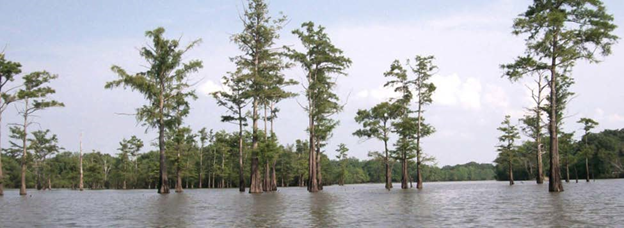
\includegraphics{images/cypress_swamp} \end{center}

This is the very first part of the book.

\chapter{Executive Summary}\label{executive-summary}

This Water Resource Inventory and Assessment (WRIA) Report for the
Felsenthal National Wildlife Refuge (NWR) summarizes the results of data
mining from national, regional, and local sources for information on
hydrology, water rights, water availability, and water quality. This
report is a compilation and summary of available and relevant
information for refuge water resources within the region of hydrologic
influence (RHI). Topics addressed within this report include facility
information, natural setting (geology, soils, climate, hydrology,
topography), and a catalog/inventory of relevant hydrologic factors
(water resources, water infrastructure, water rights). Information was
compiled from national and regional databases, geographically referenced
to the same projection, and presented within a Geographic Information
System framework.

\chapter{Introduction}\label{introduction}

The long term goal of the National Wildlife Refuge System (NWRS) Water
Resource Inventory and Assessment (WRIA) effort is to provide
up-to-date, accurate, reconnaissance-level data on water quantity and
quality to support NWRS management planning and management actions to
fulfill the NWRS mission and individual refuge purposes and management
goals. An accurate water resources inventory is essential to prioritize
issues and tasks, and to take prescriptive actions that are consistent
with the established purposes of the refuge. WRIAs evaluate significant
water resources (including rivers and streams, lakes and ponds, springs,
wetlands, and groundwater), known water quality issues, water management
infrastructure and practices, water rights, threats to water supplies,
and other water resource issues for each site.

This Water Resource Inventory (WRI) Report for Felsenthal National
Wildlife Refuge (Felsenthal NWR or ``the refuge'') summarizes available
information relevant to refuge water resources, completing the first
step of the WRIA process for the refuge. Major topics addressed in this
report include the natural setting of the refuge (topography, climate,
geology, soils, hydrology), impacts of development and climate change,
significant water resources and associated infrastructure within the
refuge, past and current water monitoring activities on and near the
refuge, water quality information, and state water use regulatory
framework. Information was compiled from publicly available reports,
databases, and geospatial datasets from federal, state, and local
agencies; published research reports; websites maintained by government
agencies, academic institutions, and non-governmental organizations; and
from files and geospatial data layers maintained by the refuge.

This WRI report is presented on two scales: intermediate (within a
Region of Hydrologic Influence (RHI) encompassing the refuge), and local
(within the NWR). The WRI is the first step in the completion of a Water
Resources Inventory and Assessment (WRIA). The inventory and assessment
process continues with data assimilation at the local level and the
assessment of key water resource issues of concern (threats or
stressors) and needs. The WRIA report will synthesize the intermediate
and local water resources inventory data and provide a summary of the
threats and needs associated with water resources for ongoing water
resource management and strategy development.

\section{Document Organization}\label{document-organization}

This WRI report is partitioned into several categories and
sub-categories according to a nationally adopted format for conducting
water resource inventory and assessments through the US Fish \& Wildlife
Service (USFWS). This document follows this same format for easy
inter-refuge operability, and is organized as follows:

\begin{itemize}
\tightlist
\item
  Facility information and habitats
\item
  Natural Setting: topography, geology, hydrogeology, soils, hydrology
  and climate
\item
  Inventory: water resources, water resource infrastructure, water
  quality, and water monitoring
\item
  Assessment: threats and needs
\end{itemize}

The WRI report contains general information and maps describing the
natural setting of the refuge. More detailed information can be found in
the inventory section about water resources, water infrastructure, water
quality, and water monitoring. The inventory also contains information
about federal and state regulations for Felsenthal NWR and the
surrounding area's water resources. Some of the information, such as
data sources and links to the information is provided in the Appendix.

\bibliography{book}


\end{document}
